\section{Theoretical Background in Reinforcement Learning}
Reinforcement learning (RL) is an approach in artificial intelligence for goal-directed learning from interaction and experience. This makes it different from the other approaches in machine learning in which the learner, the decision maker, or the so called agent, is told what to do. In reinforcement learning the agent tries out different actions in order to understand which of them generates the most reward. The reward is a special term in reinforcement learning which describes the goal in a Markov decision process (MDP) model. Roughly speaking, the MDP model would very well characterize the agent’s view of the world, the actions that it can take in the world and its goal.

Machine learning distinguishes supervised from unsupervised learning paradigms by having the supervisor indicating the correct behavior in certain generalized situations for the supervised learning and finding hidden structure in unlabeled data for the unsupervised learning. Reinforcement learning is sometimes classified as an unsupervised learning problem, because it doesn’t make use of labeled data, however it doesn’t look for structure, but tries to maximize the reward. Therefore, reinforcement learning is considered another paradigm in machine learning, according to the opinion and points of the authors R. S. Sutton and A. G. Barto of the book “An introduction to Reinforcement Learning” \cite{Sutton}. The diagram in \Cref{fig:RLandML} illustrates the relationship between machine learning and reinforcement learning.
\begin{figure}[H]
	\centering
	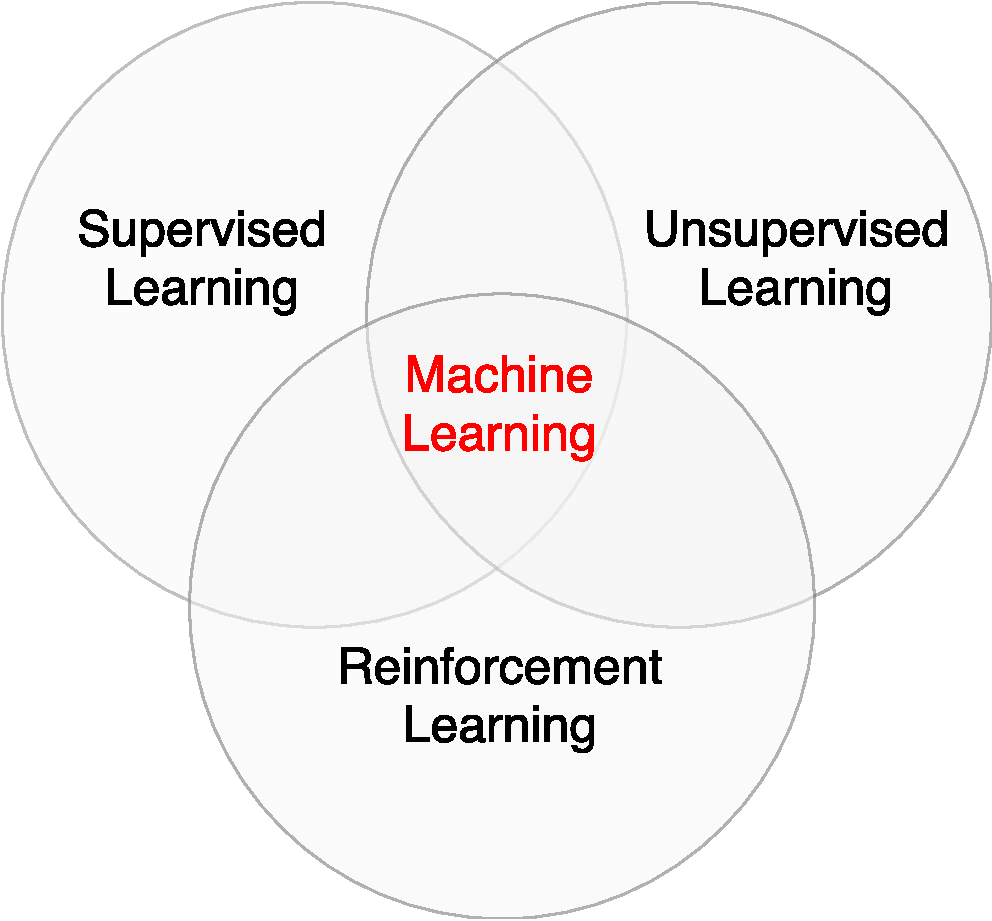
\includegraphics[width=0.7\textwidth]{Figures/RLandML}
	\caption{Reinforcement Learning and Machine Learning}
	\label{fig:RLandML}
\end{figure}
Reinforcement learning considers the problem of planning in real time decision making and the models for prediction related to planning. The interactive goal-directed agent is able to operate in an uncertain set up, make decisions despite uncertainty and predict future events. The agent is not necessarily a robot; it can be any component in a larger system in which it interacts directly with the system and indirectly with the system’s environment. The environment is everything that the agent interacts with, it is the outer world.

There is a special concern in reinforcement learning which is not present in the other machine learning approaches. It is the issue of balancing exploitation of the knowledge that the agent has and exploration of new information in order to improve the current knowledge base.

A variety of different scientific fields intersect with reinforcement learning, especially mathematics, namely, statistics and optimization, which have an important background contribution to the reinforcement learning methods. “For example, the ability of some reinforcement learning methods to learn with parameterized approximators addresses the classical “curse of dimensionality” in operations research and control theory” \cite{Sutton}. The relationship between reinforcement learning and optimization can be exemplified by the idea of maximization of the reward signal. Actually, in reinforcement learning the agent intends to maximize the reward, but not necessarily achieves the maximum. Reinforcement learning is also part of the engineering and computer science subjects. The related algorithms have a close resemblance to the biological brain systems of animals and humans due to the reward factor involved, therefore it also binds with the psychology and neuroscience fields. The diagram in \Cref{fig:RLandOther} illustrates how reinforcement learning relates to other scientific disciplines.
\begin{figure}[H]
	\centering
	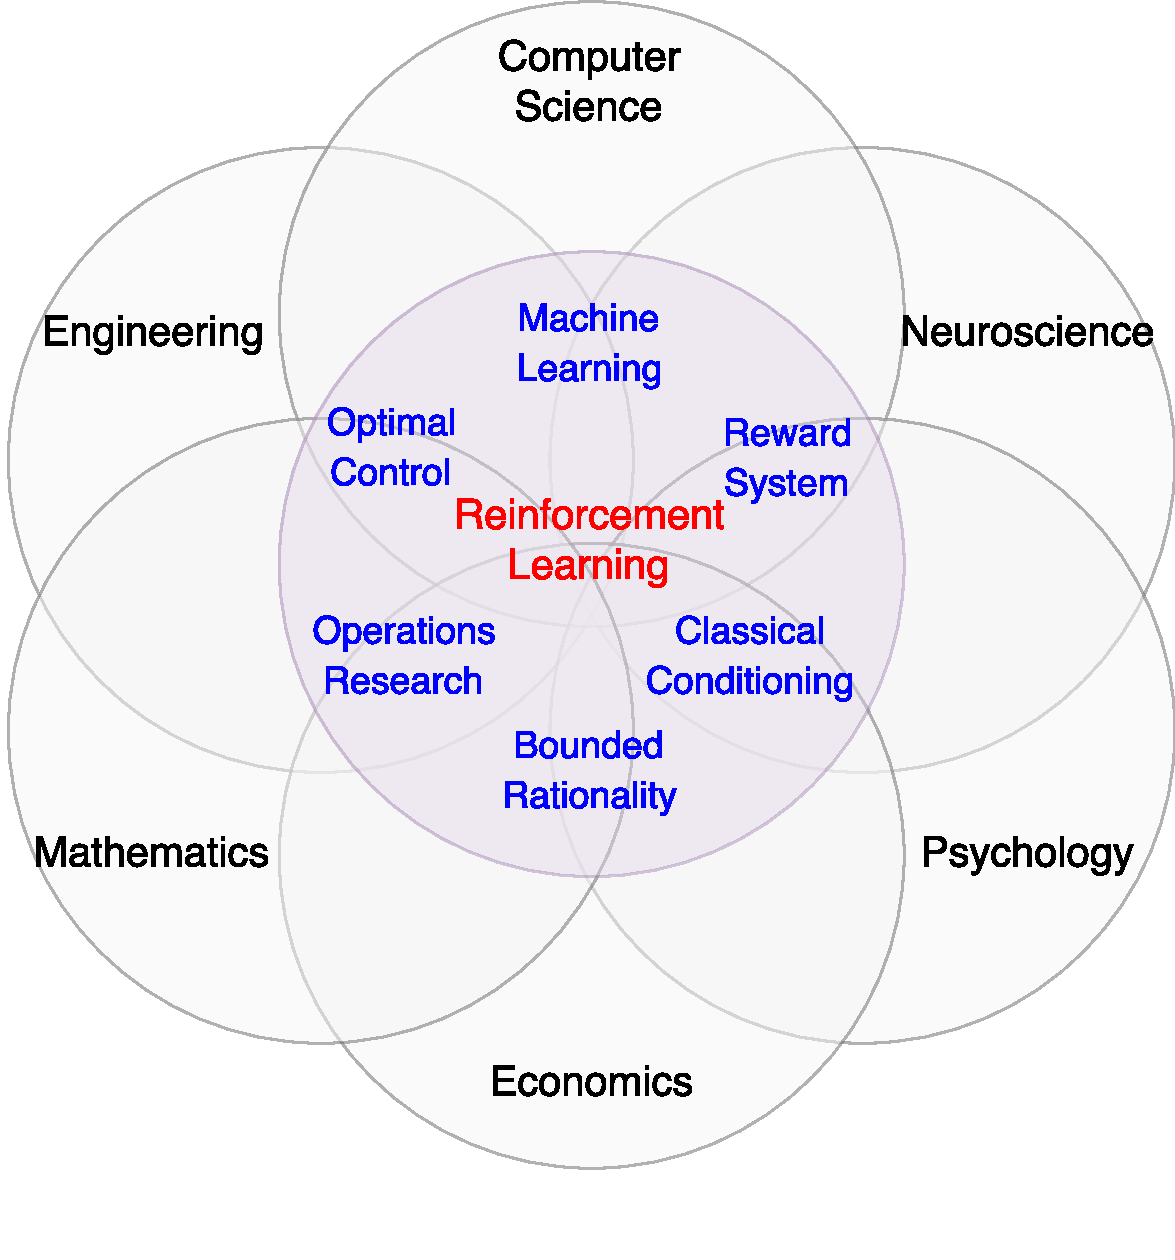
\includegraphics[width=0.7\textwidth]{Figures/RLandOther}
	\caption{Reinforcement Learning and other disciplines}
	\label{fig:RLandOther}
\end{figure}
\subsection{Elements of an RL problem}
A reinforcement learning problem contains at least one of the elements: reward signal, value function, policy, environment model.

The reward signal represents a feedback from the environment as a response to the agent’s behavior in that environment, therefore the agent cannot change the feedback that it receives, but it can behave accordingly so as to maximize the gained reward signals during its lifetime. The “reward signal defines the goal in a reinforcement learning problem” \cite{Sutton}. It serves as a problem definition and as a basis for modifying the policy.

The policy maps states to actions, so that when the agent is in a specific state, it chooses an action based on the defined policy. A policy is enough to describe the behavior of the agent and therefore, it is the core of reinforcement learning.

The value function provides values for judging about the quality of a state based on the estimated maximum reward it can yield in the long run, in contrast with the reward which expresses only the immediate advantage of being in a specific state.

The model is a representation of the environment’s behavior. In a model-free reinforcement learning (trial-and-error) problem the agent cannot plan its future, because it doesn’t have a model basis, whereas in mode-based problems the agent can plan its future actions based on the environment’s modelled behavior and expected rewards in certain states.
\subsection{Markov Decision Processes in RL}
The general reinforcement learning problem formulation has the format of a finite MDP. The interaction between the agent and environment happens at each time step of a sequence of discrete time steps, $t=0,1,2,3,...$, where at each time step $t$ the agent receives a representation of the world - a state, $S_{t}\in S$, from a set of possible states $S$, selects an action $A_{t}$ from a set of possible actions $A(S_{t})$ for the state $S_{t}$ by implementing a policy $\pi_{t}$, where $\pi_{t}(a|s)$ is the probability that $A_{t}=a$ if $S_{t}=s$, and in the next time step $t+1$ the agent receives a reward signal $R_{t+1}\in R$ from the environment ending up in a new state $S_{t+1}$ \cite{Sutton}. The diagram in \Cref{fig:AgentEnv} illustrates the interaction between the agent and the environment.
\begin{figure}[H]
	\centering
	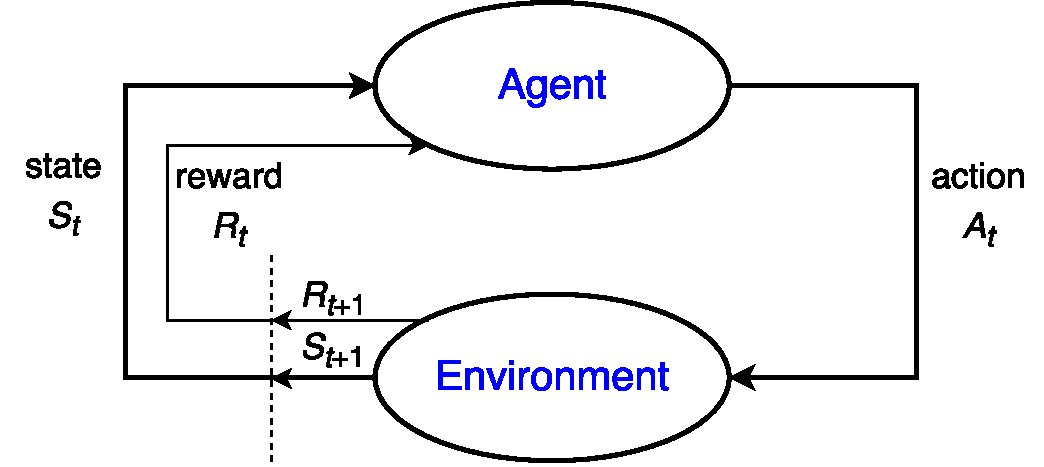
\includegraphics[width=0.7\textwidth]{Figures/Agent-EnvironmentInteraction}
	\caption{Agent - environment interaction}
	\label{fig:AgentEnv}
\end{figure}
Reinforcement learning methods provide ways to adjust the policy based on the accumulated experience with the goal of maximizing the total cumulative reward in mind. An example for representing the goal in a reinforcement learning problem like that of making a robot learn to walk would be by giving a reward on each time step proportional to the robot's forward motion. “The reward signal is your way of communicating to the robot \textit{what} you want it to achieve, not \textit{how} you want it achieved” \cite{Sutton}.

A formal definition of the cumulative reward received in the long run is expressed by the expected return $G_{t}$ which is a function of rewards sequence $R_{t+1},R_{t+2},...,R_{T}$ received after the time step $t$, where $T$ is the last time step. In order to express the return more conveniently the concept of \textit{discounting} is introduced which determines the current value of the future rewards. The formula generalized for both episodic and continuing tasks is the following: 
\begin{equation}
G_{t}=R_{t+1}+\gamma R_{t+2}+\gamma ^2R_{t+3}+...=\sum_{k=0}^{T-t-1}\gamma ^kR_{t+k+1}, 
\end{equation}
where $\gamma$ is the discount rate, $0\leq \gamma\leq1$. In the case of episodic tasks where there is a terminal state after some time steps, $\gamma=1$. For the cases in which the process is continuous and the final step is infinite, $T=\infty$. 

With the discounting factor, the reward received after $k$ time steps has the value "$\gamma ^{k-1}$ times what it would be worth if it were received immediately" \cite{Sutton}. In the extreme point where $\gamma=0$, it is said that the agent is myopic, because it only maximizes over the immediate rewards and not the future rewards, whereas if $\gamma$ is closer to $1$ the agent is farsighted and sees far into the future considering the future rewards when picking actions.

The \textit{state} that has the Markov property represents all the useful information in order to make a sufficient statistic for the future. With Markov states we have the best possible basis for choosing action \cite{Sutton}. The environment's feedback at time step $t+1$ after a particular action was taken at time step $t$ depends on the events happened before. If the state has the Markov property instead, then the feedback of the environment depends only on that state, because that state represents all the previous events. In this case the one step environment dynamics of a finite MDP can be expressed by the following formula:
\begin{equation}\label{psrsa}
p(s',r|s,a)=Pr\left \{ S_{t+1}=s',R_{t+1}=r|S_{t}=s,A_{t}=a \right \}
\end{equation}
Based on the formula presented in (\ref{psrsa}) we can also compute the expected rewards for state-action pairs \cite{Sutton},
\begin{equation}
r(s,a)=\mathop{{}\mathbb{E}}\left [ R_{t+1}|S_{t}=s,A_{t}=a \right ]=\sum_{r\in R}r\sum_{s'\in S}p(s',r|s,a)
\end{equation}
the \textit{state-transition probabilities}
\begin{equation}
p(s'|s,a)=Pr\left \{ S_{t+1}=s'|S_{t}=s,A_{t}=a \right \}=\sum_{r\in R}p(s',r|s,a)
\end{equation}
and the expected rewards for state-action-next-state triples,
\begin{equation}
r(s,a,s')=\mathop{{}\mathbb{E}}\left [ R_{t+1}|S_{t}=s,A_{t}=a,S_{t+1}=s' \right ]=
\frac{\sum_{r\in R}rp(s',r|s,a)}{p(s'|s,a)}
\end{equation}
Value functions estimate how good it is to be in a specific state given the expected return and the policy.

The \textit{state-value function} for policy $\pi$, $v_{\pi }$ expresses the expected value of a random variable given the followed policy $\pi$ at any time step $t$:
\begin{equation}
v_{\pi }(s)=\mathop{{}\mathbb{E}_{\pi}}\left [G_{t}|S_{t}=s \right ]=\mathop{{}\mathbb{E}_{\pi}}\left [ \sum_{k=0}^{\infty}\gamma ^kR_{t+k+1} |S_{t}=s\right ]
\end{equation}

The \textit{action-value function} for policy $\pi$, $q_{\pi }$ is the value of taking an action $a$ in a state $s$ while following the policy $\pi$:
\begin{equation}
q_{\pi }(a,s)=\mathop{{}\mathbb{E}_{\pi}}\left [G_{t}|S_{t}=s,A_{t}=a \right ]=\mathop{{}\mathbb{E}_{\pi}}\left [ \sum_{k=0}^{\infty}\gamma ^kR_{t+k+1} |S_{t}=s,A_{t}=a\right ]
\end{equation}

Value functions have the property of being expressed recursively. The recursive representation is actually the \textit{Bellman equation} and it's solution is the value of $v_{\pi }$. It is like a look ahead procedure, where the value of a current state is evaluated by looking ahead at the values that future states can offer. "The Bellman equation averages over all the possibilities, weighting each by its probability of occurring. It states that the value of the start state must equal the (discounted) value of the expected next state, plus the reward expected along the way" \cite{Sutton}:
\begin{equation}\label{StateValueFunction}
v_{\pi }(s)=\mathop{{}\mathbb{E}_{\pi}}\left [G_{t}|S_{t}=s \right ]=\sum_{a}\pi(a|s)\sum_{s',r}p(s',r|s,a)\left [ r+\gamma v_{\pi }(s') \right ]), \forall s\in S
\end{equation}
The Bellman equation represents the basis of different ways of computing, approximating, and learning $v_{\pi }$ \cite{Sutton}.

In finite MDPs, an \textit{optimal policy} $\pi_{*}$ is the policy for which its expected return for all the states is greater than or equal to the expected return of all the other policies. There can be many policies that are optimal due to their \textit{state-value function}, which evaluates the same for all the optimal policies:\begin{equation}
v_{*}(s)=\max_{\pi}v_{\pi}(s), \forall s\in S
\end{equation}

Analogically, the \textit{optimal action-value function} is formed:
\begin{equation}
q_{*}(s,a)=\max_{\pi}q_{\pi}(s,a), \forall s\in S , a \in A(s)
\end{equation}

The \textit{Bellman optimality equation} for $v_{*}$ is the value of a state on the optimal policy basis, which is the same as the expected return of the best action for that state \cite{Sutton}:
\begin{equation}\label{BellmanOptimalityVstar}
\begin{split}
v_{*}(s)&=\max_{a \in A(s)}q_{\pi*}(s,a) \\
&=\mathop{{}\mathbb{E}}\left [ R_{t+1} + \gamma v_{*}(S_{t+1})|S_{t}=s, A_{t}=a  \right ] \\
&=\max_{a \in A(s)}\sum_{s',r}p(s',r|s,a)\left [ r+\gamma v_{*}(s') \right ]
\end{split}
\end{equation}

And the \textit{Bellman optimality equation} for $q_{*}$ is the following:
\begin{equation}\label{BellmanOptimalityQstar}
\begin{split}
q_{*}(s,a)&=\mathop{{}\mathbb{E}}\left [ R_{t+1} + \gamma \max_{a'}q_{*}(S_{t+1},a')|S_{t}=s, A_{t}=a  \right ] \\
&=\sum_{s',r}p(s',r|s,a)\left [ r+\gamma\max_{a'}q_{*}(s',a') \right ]
\end{split}
\end{equation}

The Bellman optimality equation generates a system of $N$ nonlinear equations, where $N$ is the number of states. It can be simply solved by applying some nonlinear methods when the system dynamics ($p(s',r|s,a)$) are known. The solution to the Bellman optimality equation helps in defining the optimal policy; e.g. one can, at any state, choose the action that corresponds to the maximum return, which is also valid in the long term, because the values take into account the reward consequences of all possible future behavior options \cite{Sutton}. In the case of the action-value pairs, if the system's dynamics are unknown, then the actions would still be optimal, because the agent would choose the actions that would maximize $q_{*}$.

\subsection{Solution methods}
The solution methods for the reinforcement learning problem can be divided into two groups, \textit{tabular} and \textit{approximate}. The tabular solution methods find exact, optimal solutions and are more suitable when the states and actions space is rather small, while the approximate solution methods provide approximate solutions and it is applicable to large spaces problems.

The process of \textit{generalized policy iteration} (GPI) provides a good way of getting insight into the methods of RL. GPI employs a sequence of interleaved policy evaluations and policy improvements, where the given policy is evaluated, for example, by computing it's value function, and the policy is improved by using the value function. This process is proven to converge to an optimal policy and value function for the classical dynamic programming methods. GPI represents the way that almost all RL methods work. The \Cref{fig:GPI} illustrates the process better.
\begin{figure}[H]
	\centering
	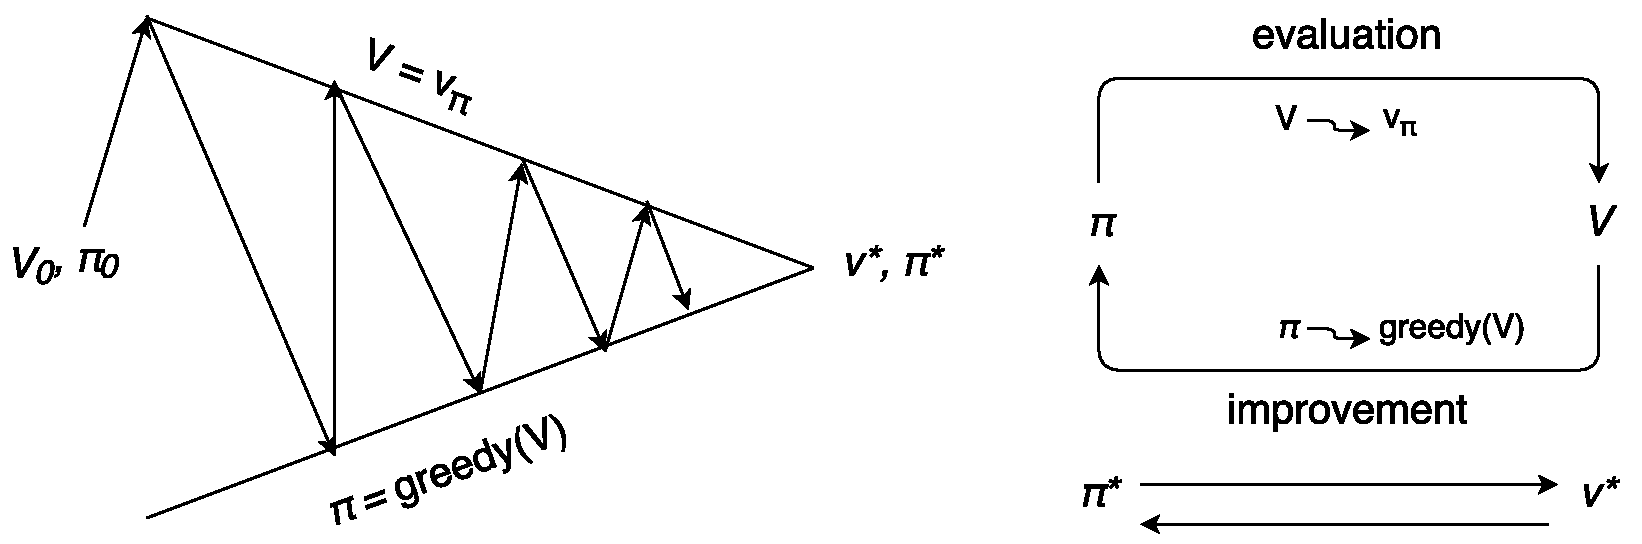
\includegraphics[width=0.9\textwidth]{Figures/GPI}
	\caption{Generalized Policy Iteration}
	\label{fig:GPI}
\end{figure}
Another way of presenting the GPI is in terms of \textit{prediction} and \textit{control}. The prediction problem is referring to policy evaluation or the estimation of $v_{\pi}$ for a given policy $\pi$, whereas the control problem is referring to the actual optimal policy $\pi_{*}$ seeking.

The relevant notions for describing the methods of RL are \textit{backup} and \textit{bootstrap}. A \textit{full backup} updates a state's value on the basis of the next states estimated values. \textit{Bootstrapping} refers to the idea of updating estimates based on other estimates.

Usually, the RL solution methods vary in the way they approach the prediction and control problems, and also in whether they need a model of the environment or they use bootstrapping.

\subsubsection{Tabular solution methods}
The tabular solution methods include three important classes of methods for solving the finite MDP: \textit{Dynamic Programming} (DP), \textit{Monte Carlo} (MC) and \textit{Temporal-Difference} (TD) learning.

Dynamic programming uses the Bellman optimality equations \ref{BellmanOptimalityVstar} and \ref{BellmanOptimalityQstar} as update functions for \textit{policy iteration} which yields a sequence of monotonically increasing value functions and policies: ${\pi}_{0}\overset{E}{\rightarrow}v_{{\pi}_{0}}\overset{I}{\rightarrow}{\pi}_{1}\overset{E}{\rightarrow}v_{{\pi}_{1}}\overset{I}{\rightarrow}{\pi}_{2}\overset{E}{\rightarrow}...\overset{I}{\rightarrow}{\pi}_{*}\overset{E}{\rightarrow}v_{*}$, where $E$ stands for evaluation and $I$ - for improvement. That is, an arbitrary fixed policy is evaluated by computing it's state-value function and is improved by computing it's state-action value function. If the state-action value function of choosing an action $a \neq \pi(s)$ is greater than the state-value function $v_{\pi}(s)$, then the policy is changed to a new policy. The formula for getting a new policy is given by \ref{PolicyImprovement}:
\begin{equation}\label{PolicyImprovement}
\begin{split}
\pi'&=\arg\!\max_{a}q_{\pi}(s,a)\\
&=\arg\!\max_{a}\mathop{{}\mathbb{E}}\left [ R_{t+1} + \gamma v_{\pi}(S_{t+1})|S_{t}=s, A_{t}=a  \right ] \\
&=\arg\!\max_{a}\sum_{s',r}p(s',r|s,a)\left [ r+\gamma v_{\pi}(s') \right ]
\end{split}
\end{equation}

Unlike the DP methods, the Monte Carlo and the temporal-difference solution methods don't require the model parameters to be known in advance, meaning that no previous knowledge about the environment is needed and that the agent learns exclusively from it's \textit{experience} (sampled states, actions, rewards). The MC method doesn't bootstrap, whereas TD does use bootstrapping, like the DP methods.

MC differs from DP in the way it handles the prediction problem. It uses averages over the sampled returns from a specific state on episode-by-episode basis in order to learn over multiple observed returns the value function, whereas in DP the value function was computed from the knowledge of the MDP. The policy evaluation is performed by computing the value of the state-action pairs for the visited states over an episode. The policy improvement is performed by adjusting the policy closer to the action with the maximal value for a specific state.

Because MC doesn't make all the possible actions, it is required to employ some kind of guarantee for exploration. This can be achieved by assigning nonzero probabilities for all the actions in order to make sure they are going to be picked eventually. This is called \textit{exploring starts}. A better approach are the \textit{on-policy} and \textit{off-policy} methods. 

On-policy methods have probabilities greater than zero for all their actions, meaning that they have \textit{soft} policies. The policies in on-policy methods become closer to an optimal deterministic policy in time. The exploring starts is an example of on-policy method. Another example would be an $\epsilon$-greedy policy where the best action is chosen with the probability $1-\epsilon$ and, sometimes, another random action is chosen with the probability $\epsilon$.

Off-policy methods use 2 policies: a \textit{target policy} $\pi$ which is a deterministic policy, like the one presented in the on-policy methods, and a \textit{behavior policy} $\mu$ which is stochastic in states and generates data by exploring. Both policies have non zero probabilities that ensures the coverage property. Off-policy methods can be implemented with \textit{importance sampling} technique. The importance sampling technique computes an importance sampling ratio based on the relative probabilities of the returns' trajectories from both policies and it is used for weighting the returns for learning the value function.

TD differs from DP also in the way it handles the prediction problem. TD makes an estimate of the value function after each time step by sampling expected values and using current value estimates. Therefore, TD is a combination of MC sampling and DP bootstrapping. The simplest TD method is also called \textit{TD(0)}. The update function for TD(0) \ref{PolicyEvaluationTD0} is the following:
\begin{equation}\label{PolicyEvaluationTD0}
V(S_{t})\leftarrow V(S_{t})+\alpha \left [ R_{t+1}+\gamma V(S_{t+1})-V(S_{t}) \right ]
\end{equation}
If we compare the MC target with the TD target, the MC target has $G_{t}$ instead of the immediate reward and the value estimate of the next state. The square brackets represents the TD error, or the MC error in the MC update function. An important observation is that the sum of the time steps TD errors gives an episode of MC error.

For solving the control problem with TD(0) and on-policy methods, action-value functions are used instead of the value function that we've just seen. A "transition from one action-state pair to another" \cite{Sutton} yields a quintuple of the form $(S_{t}, A_{t}, R_{t+1}, S_{t+1}, A_{t+1})$, \textit{Sarsa}, which is the name of the algorithm. Therefore, for evaluating the policy, an estimation of the $q_{\pi}$ is required and for improving the policy, $\pi$ is greedily adjusted closer to it's $q_{\pi}$.

An notable off-policy TD(0) algorithm is \textit{Q-learning}. It is an off-policy method because it learns the optimal action-value function $q_{\pi*}$ independent of the policy. The action is picked greedily according to the estimated $Q$ but the $Q$ is updated based on the action that produces maximal value. 

A slight change into the update function of $Q$ would lead us to the \textit{Expected Sarsa} algorithm. The change is that instead of maximizing over the next action-value pairs, the expected return is taken which considers the probabilities of making those actions according to the current policy. Expected Sarsa is a better algorithm in comparison with Sarsa and Q-learning.

The MC and TD methods are extended into more complicated and powerful forms to achieve better performance, but the essence of these methods perpetuates in all the other algorithms. An idea about combining these two methods would be to unify them under \textit{n-step} algorithms instead of the extreme one time step in TD(0) and a whole episode in MC, or perform additions of other features like eligibility traces and model learning.
	
\subsubsection{Approximate solution methods}
The approximate solution methods are an extension to the tabular solution methods for huge states spaces problems. In this type of problems, the goal is to find a good approximate solution under the condition of restricted computational resources. Because almost every visited state is seen for the first time, every state being so unique, the agent needs to be able to make sense of it and, therefore, usefully generalize the information it gets. This is possible thanks to function approximation. “Function approximation is an instance of supervised learning, the primary topic studied in machine learning, artificial neural networks, pattern recognition, and statistical curve fitting” \cite{Sutton}.

The value function is represented by a function of a weights vector instead of a table. The approximated value function looks like $\hat{v}(s,\theta)\approx v_{\pi}(s)$, which can be translated into words as the approximated value of a state $s$ given the weights vector $\theta$. The value function can be an artificial neural network with multiple layers where the weights are adjusted and learned. A single adjustment of the weights would change the value appreciation for all the states. This process is difficult to follow and track, but it is more powerful. This would create the necessary \textit{generalization} for the agent to learn from it and apply knowledge in multiple similar, but different states.

With function approximation different supervised machine learning methods can be applied to simulate outputs for a set of inputs. The estimated value of a state $s$ should look more like a number $g$ and this relation $s \mapsto g$ can be used as a training example for supervised learning which would learn to predict values for other states. $s \mapsto g$ is referred to as a back-up, where $s$ is the state backed-up and $g$ is the backed-up value or target. For example, the target in MC methods is the return $G_{t}$, so the back-up is $S_{t} \mapsto G_{t}$, whereas the back-up in TD(0) is $S_{t} \mapsto R_{t+1}+\gamma\hat{v}(S_{t+1}, \theta_{t}) $.

Some common ways of doing function approximation are based on gradient principles. For any $\theta$ the function approximator can not exactly represent all the states and examples, therefore the idea is to find a balance - a weights vector that would, as close as possible, represent all the states. A performance measure could be defined by the \textit{mean squared value error} (MSVE) shown below (\Cref{MSVE}). The error represents the squared difference between the estimated value $\hat{v}(s,\theta)$ and the actual value $v_{\pi}(s)$, whereas the $d(s)$ represents the weight or the distribution of the error for a state $s$. The goal would become the minimization of MVSE.
\begin{equation}\label{MSVE}
MVSE(\theta)=\sum_{s\in S} d(s) \left [ v_{\pi}(s) - \hat{v}(s,\theta) \right ]^{2}
\end{equation}

For each training example the \textit{Stochastic Gradient Descent} (SGD) method would update the weights so that they minimize the error in that example, \Cref{SGD}:
\begin{equation}\label{SGD}
\theta_{t+1}=\theta_{t}+\alpha \left [ v_{\pi}(S_{t}) - \hat{v}(S_{t},\theta_{t}) \right ]\nabla\hat{v}(S_{t},\theta_{t})
\end{equation}
In the MC method, the target is an unbiased estimate of $v_{\pi}(s)$, therefore the SGD would be a good choice to be applied, because it would converge to a locally optimal solution for the value function. In the bootstrapping cases, however, SGD is not the best choice, because the targets usually depend on the weights vector that is changing and causing the targets to be biased. These methods are called \textit{semi-gradient} methods instead, and they converge in the linear case.

Linear methods have feature vectors $\phi(s)$ that represent the state. The inner product between the feature vector $\phi(s)$ and the weights $\theta$ makes up the function approximation $v_{\pi}(s,\theta)$. In such a situation the SGD method can be applied and get an even simpler form of weights update. This is proven to converge to a global optimum, including for the MC linear function approximation version and the semi-gradient TD(0) with an additional theorem.

Nonlinear methods for function approximation involve \textit{artificial neural networks} (ANNs). ANNs are the product of inspiration from the neural networks in the brains of animals and humans. Their properties and functionality have been successfully replicated in ANNs. An ANN is a layered structure of neurons which has minimum one input layer and one output layer. Each layer has a number of units (neurons) that are connected to the units in another layer. The connections are assigned weights that are used for the unit's \textit{activation}. In order to perform activation, a weighted sum of it's inputs is computed at each unit and then passed to an activation function to produce output. There are different activation functions, though, and the choice depends on the type of problem. Also, in dependence of the structure of the network, there are different types of ANNs. For example, a simple case of feedforward ANN with an input layer of 4 units, 2 hidden layers, and an output layer with 2 units is presented in the \Cref{fig:feedforward}:
\begin{figure}[H]
	\centering
	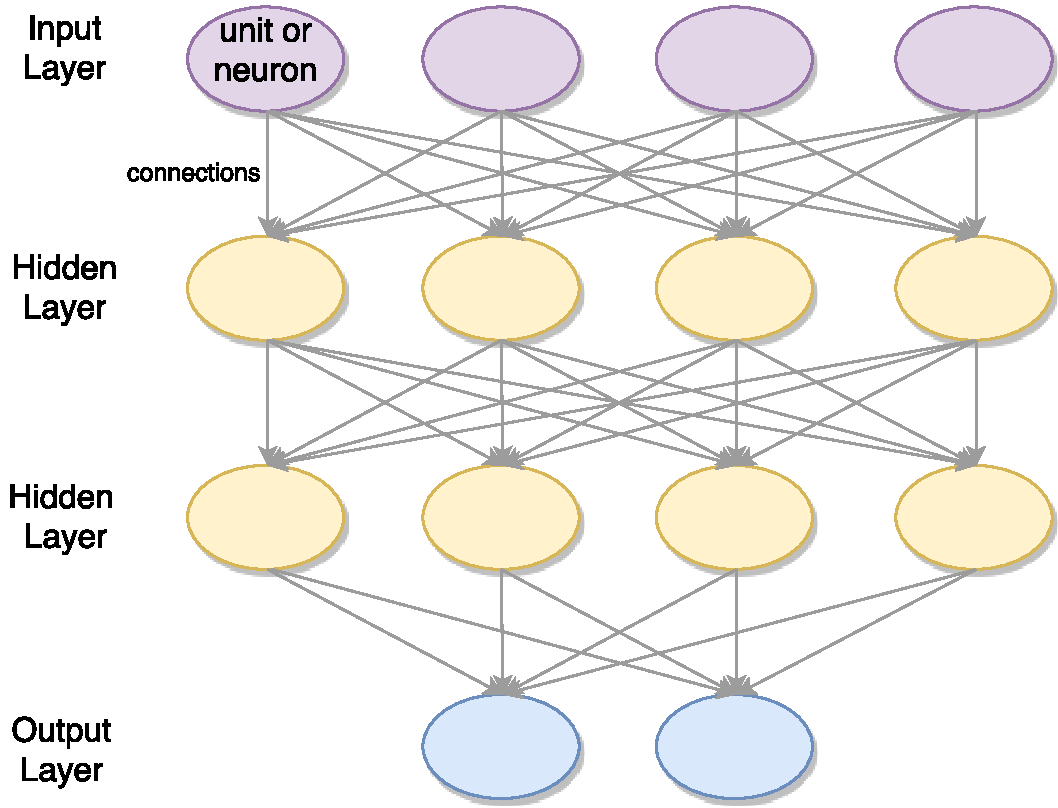
\includegraphics[width=0.7\textwidth]{Figures/Feedforward}
	\caption{Feedforward ANN}
	\label{fig:feedforward}
\end{figure}
RL uses ANNs in it's most representative applications and especially deep ANNs.

The Policy Gradient Methods learn a \textit{parameterized policy} and makes it possible to select the action without calculating the value function. So, in a given state $s$, at a given time $t$, the agent selects an action $a$ based on the weights vector ${\theta}$ of the policy: ${\pi}(a|s,{\theta})=Pr\{A_{t}=a|S_{t}=s,{\theta}_{t}={\theta}\}$. The policy weights are learned according to an approximate gradient of a performance indicator ${\eta}({\theta})$ with respect to the policy weights which tries to maximize the performance. 

The methods that use both policy and value approximations are named actor-critic methods, where the actor estimates the policy weights vector for choosing an action and the critic estimates the value weights for providing the information about the quality of a state the agent ends up in after making the action according to the policy.